\section{Results}
\subsection{Matched 90-day comparison}
The coupled model produced a lower-density interior than Fisher--KPP, despite a similar spatial extent at the lower density threshold (Figure~\ref{fig:fields}). At day 90, M2 contained \CoupledCells{} billion viable cells versus \ReferenceCells{} billion in M0, a \CellReduction\% reduction. The respective volumes with $c/K\geq0.2$ were \CoupledVolume{} and \ReferenceVolume{} mL, differing by only \VolumeReduction\%. In contrast, the volume with $c/K\geq0.8$ was zero in M2 and 1.944 mL in M0. Peak viable densities were \CoupledPeak{} and \ReferencePeak{} times $K$, respectively.

\begin{figure}[p]
\centering
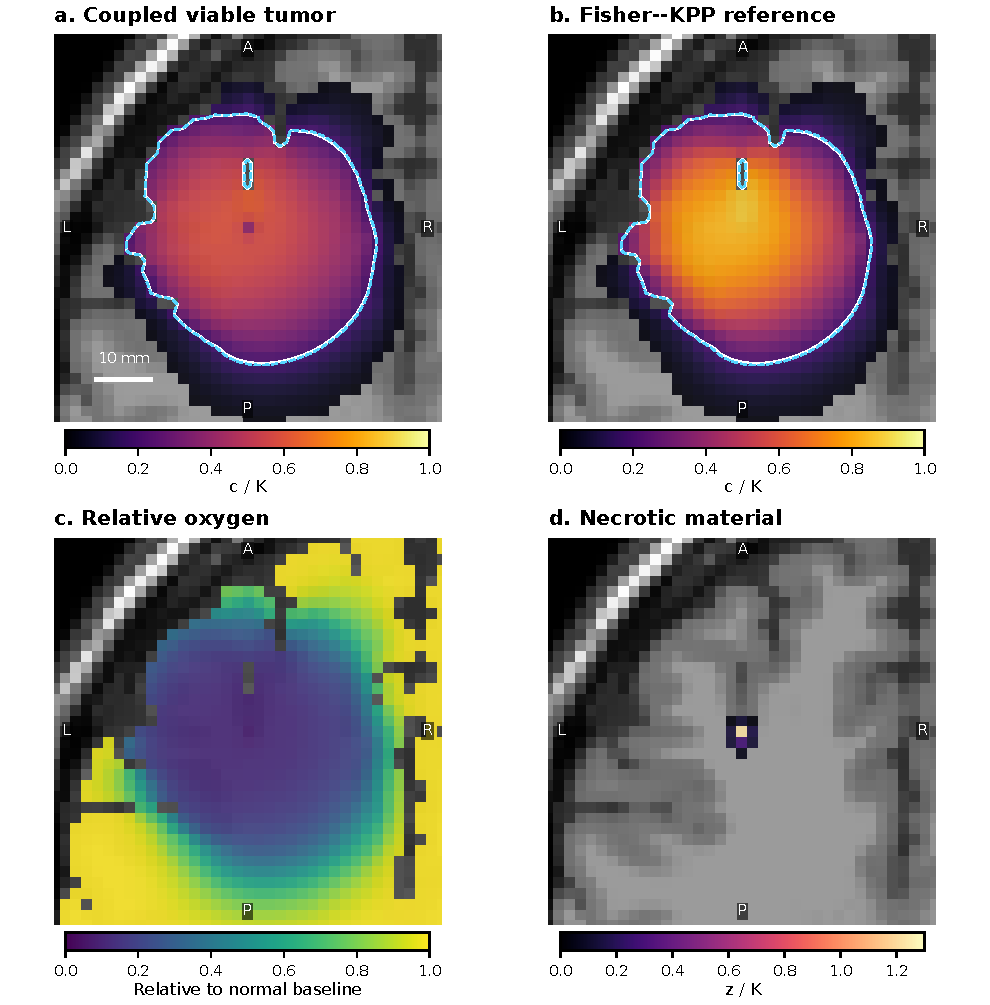
\includegraphics[width=0.94\textwidth]{figures/day90_fields.pdf}
\caption{Day-90 fields in the matched primary simulations. Axial views at RAS $z=30$ mm show a $72\times72$ mm region, with the original 2 mm simulation pixels retained. Viable density and the reference share the same $0$--$1$ color scale; oxygen is relative to the normal baseline. Necrotic material is shown over $0$--$1.3$ without clipping its peak at one. White solid and cyan dashed contours mark $c/K=0.2$ in M2 and M0, respectively. Tumor/necrosis overlays below 0.02 of $K$ are transparent for display only. The scale bar is 10 mm. These thresholds and colors have no calibrated correspondence to MRI contrast.}\label{fig:fields}
\end{figure}

Minimum tissue oxygen in M2 was \MinimumOxygen{}. Necrotic material totaled \NecroticCells{} million cell equivalents, with $z/K\geq0.2$ occupying \NecroticVolume{} mL, or three 2 mm voxels. Low-oxygen volume ($o<0.1$) was 0.104 mL. The dense initial seed was already oxygen limited; this experiment therefore does not demonstrate the spontaneous emergence of a macroscopic necrotic core from a dilute initial tumor. The tiny thresholded focus is not a resolved anatomical cavity. Moreover, the maximum $z/K=\MaximumNecrosis{}$ exceeds one, as permitted by the cell-equivalent formulation.

The viable-count gap between M0 and M2 was \CellGapMillion{} million cells. Only \NecroticCells{} million cell equivalents were stored as necrotic material. With no clearance, the remaining \BirthGapMillion{} million difference in live-plus-dead burden is attributable to reduced cumulative births in the discrete balance. Thus, in this case, the smaller viable burden mainly reflects inhibited proliferation rather than death transfer.

\subsection{Controlled model ablations}
Table~\ref{tab:ablations} and Figure~\ref{fig:curves} separate growth inhibition, death transfer and the chosen supply feedback. Removing hypoxic death (M1) increased day-90 viable count by approximately 0.14\% relative to M2. In contrast, removing burden-dependent suppression of oxygen supply ($\alpha=0$) gave 2.829 billion viable cells, approximately 0.62\% below M0. Its minimum oxygen, 0.2245, remained above the death threshold, and no necrotic material formed. The supply closure therefore has a much larger effect on this particular comparison than the death term. This finding is conditional on the assigned parameters and dense seed, and does not establish the closure biologically.

\begin{table}[tbp]
\centering\small
\caption{Day-90 outcomes for 2 mm model ablations with a maximum 0.25-day step. $V_{0.2}$ and $V_{0.8}$ are viable-density threshold volumes in mL. Oxygen and necrotic state variables are absent from M0, indicated by dashes.}\label{tab:ablations}
\setlength{\tabcolsep}{4pt}
\begin{tabularx}{\textwidth}{Yrrrrr}
\toprule Model & $N_c/10^9$ & $V_{0.2}$ & $V_{0.8}$ & $\min o$ & $N_z/10^6$\\\midrule
\AblationRows
\bottomrule
\end{tabularx}
\end{table}

Setting uptake to zero ($\beta=0$) maintained $o=1$, yielded no necrotic material and reproduced the M0 solution. The largest final density discrepancy divided by $K$ was below $10^{-5}$, consistent with finite-precision differences between the numerical paths. This is a limiting-case verification, not an independent biological comparison.

\begin{figure}[p]
\centering
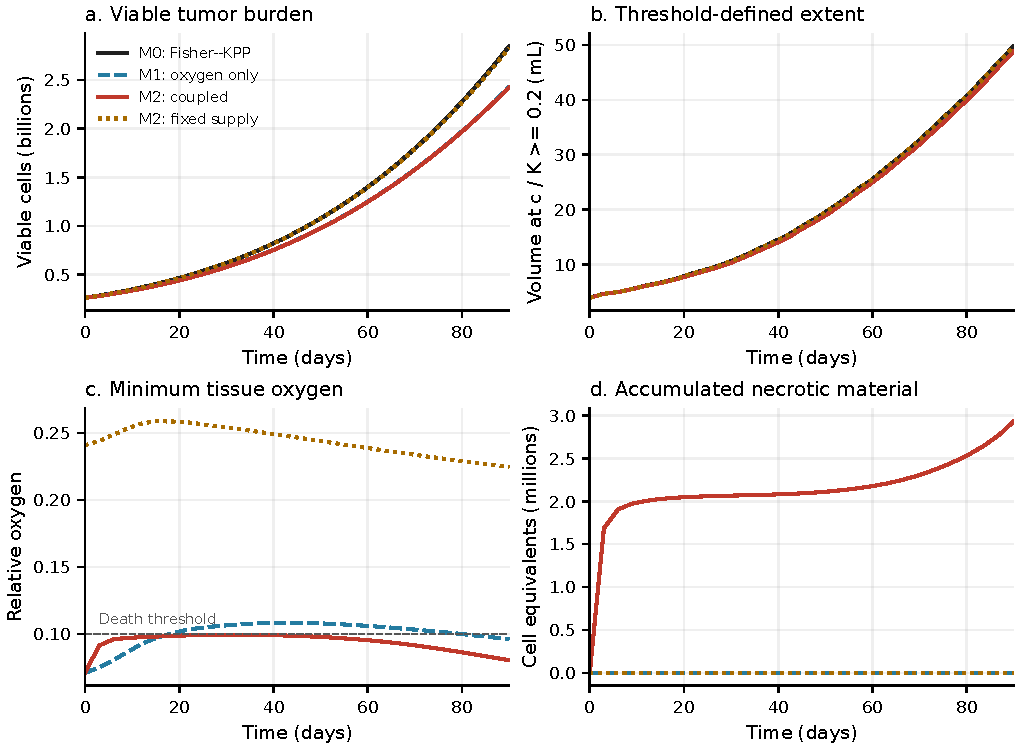
\includegraphics[width=\textwidth]{figures/timecourses.pdf}
\caption{Time courses for the matched reference and selected ablations. Panels show viable cell count, threshold-defined viable volume, minimum tissue oxygen and necrotic cell equivalents. M0 has no oxygen or necrosis state; these curves are consequently omitted. The dashed horizontal line in panel c marks $\theta_d=0.1$. M1 and M2 burden curves nearly overlap. All curves are deterministic simulations with assigned parameters; they are not measurements, replicate averages or uncertainty intervals.}\label{fig:curves}
\end{figure}

\subsection{Numerical verification and resolution dependence}
The software test suite passed all \TestCount{} tests. Checks include analytical logistic behavior, diffusion conservation, boundary behavior, positivity, death-transfer balance, oxygen bounds and model limits (Appendix~\ref{app:numerics}). These results verify implemented properties without validating the biological assumptions.

At 2 mm, reducing the maximum time step from 0.25 to 0.125 day decreased the final relative $L^2$ difference in viable density against the 0.0625-day calculation from 0.1270\% to 0.0423\%. Corresponding necrotic-field differences decreased from 4.238\% to 1.386\%. The relative oxygen differences were 0.0129\% and 0.0043\%. These comparisons support temporal refinement of the implemented scheme; a finite reference calculation does not provide an exact error or establish an asymptotic convergence order.

\begin{table}[tbp]
\centering\small
\caption{Day-90 outcomes under temporal and anatomical-grid refinement for M2. $h$ is voxel spacing in mm and $\Delta t$ is the maximum step in days. The 1 mm run changes both the numerical mesh and the discretized tissue boundaries.}\label{tab:refinement}
\begin{tabular}{rrrrrr}
\toprule $h$ & $\Delta t$ & $N_c/10^9$ & $N_z/10^6$ & $\min o$ & $\max(z/K)$\\\midrule
\RefinementRows
\bottomrule
\end{tabular}
\end{table}

The native 1 mm calculation contained 2.452 billion viable cells, compared with 2.878 billion in its matched M0 reference, a \NativeCellReduction\% reduction. This relative reduction is similar to the primary result. However, minimum oxygen fell to \NativeMinimumOxygen{}, the necrotic-equivalent count increased to 3.607 million and peak $z/K$ rose to \NativeMaximumNecrosis{}. The necrotic threshold occupied 0.032 mL (32 native voxels), while low-oxygen volume was 0.027 mL. These local quantities are sensitive to spatial resolution and to the discrete anatomy. Neither grid resolves the assigned 0.2 mm oxygen length; spatial convergence of the oxygen--necrosis subsystem has not been demonstrated.

\subsection{Homogeneous parameter recovery and uncertainty}\label{sec:recovery_results}
In the separate homogeneous experiment, all three initial guesses converged to the same fit at the reported precision. Estimated diffusion was \RecoveryDEstimate{} mm$^2$/day and proliferation was \RecoveryRhoEstimate{} day$^{-1}$, relative errors of \RecoveryDRelativeError\% and \RecoveryRhoRelativeError\%, respectively (Table~\ref{tab:recovery}). Both known values lay within the local and bootstrap marginal 95\% intervals. The log-parameter correlation was \RecoveryCorrelation{}, indicating that uncertainty in the two rates should be propagated jointly. No primary or replicate fit reached a bound or failed. Agreement across starts and finite sensitivity singular values support local estimation for this experiment; they do not establish global identifiability under unknown initialization.

\begin{table}[tbp]
\centering\small
\caption{Recovery from the first three noisy scans of the homogeneous phantom. Local intervals use the known-noise residual Jacobian; bootstrap intervals are percentiles of \RecoveryBootstraps{} refits. Intervals are marginal, frequentist and conditional on known initialization and imaging assumptions.}\label{tab:recovery}
\setlength{\tabcolsep}{4pt}
\begin{tabularx}{\textwidth}{lrrYY}
\toprule Parameter & Known & Estimate & Local 95\% CI & Bootstrap 95\% CI\\\midrule
\RecoveryRows
\bottomrule
\end{tabularx}
\end{table}

Across \RecoveryTrials{} independent noise realizations, local intervals covered $D$ in \RecoveryDCoverageCount/\RecoveryTrials{} trials and $\rho$ in \RecoveryRhoCoverageCount/\RecoveryTrials{} trials (Table~\ref{tab:recovery_coverage}; Figure~\ref{fig:recovery}). The exact binomial intervals include the nominal 95\% rate and remain broad. The observed 98.3\% and 100\% fractions therefore neither establish exact calibration nor imply guaranteed coverage. The study varies measurement noise at one fixed biology, initialization and imaging setting, rather than sampling a virtual patient population. The time-zero-only control was correctly rejected as locally unidentifiable.

\begin{table}[tbp]
\centering\small
\caption{Independent repeated-noise recovery audit of local 95\% intervals. Bias and RMSE retain the units in the parameter column. The last column quantifies sampling uncertainty in empirical coverage, not uncertainty in an individual parameter estimate.}\label{tab:recovery_coverage}
\setlength{\tabcolsep}{4pt}
\begin{tabularx}{\textwidth}{lrrYY}
\toprule Parameter & Bias & RMSE & Coverage & Binomial 95\% CI\\\midrule
\RecoveryCoverageRows
\bottomrule
\end{tabularx}
\end{table}

\begin{figure}[p]
\centering
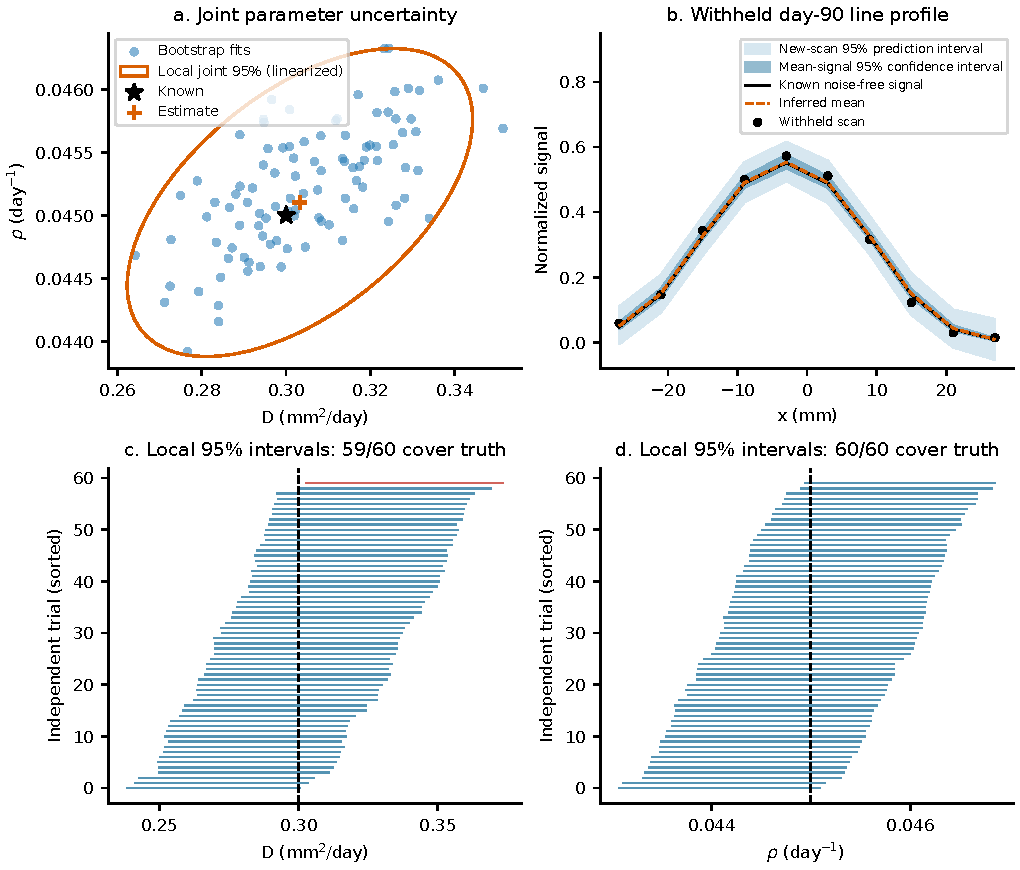
\includegraphics[width=\textwidth]{figures/synthetic_recovery.pdf}
\caption{Synthetic recovery and conditional uncertainty. (a) Joint bootstrap estimates and a local joint 95\% ellipse, linearized into physical units. The star marks the known rates. (b) A day-90 line profile through the nearest observation-voxel centers to the seed's $y,z$ coordinates. The darker mean-signal confidence band accounts for parameter uncertainty; the lighter new-scan prediction band also includes independent noise. Both are pointwise intervals. (c,d) Local marginal 95\% intervals for the \RecoveryTrials{} independent noise realizations, sorted by fitted rate. Red denotes a missed known value; the dashed line is ground truth. These trials audit local intervals, not bootstrap coverage or clinical variability.}\label{fig:recovery}
\end{figure}

\subsection{Withheld homogeneous forecasts and numerical discrepancy}
Day-75 and day-90 predictions used no observations beyond day 60. Whole-image RMSE against the known noise-free signal was $4.72\times10^{-4}$ and \RecoveryDayNinetyRMSE{}, respectively, while RMSE against the withheld noisy images was approximately the 0.03 noise standard deviation (Table~\ref{tab:recovery_forecast}). The 95\% new-scan prediction intervals contained 94.0\% and 94.6\% of the withheld voxel measurements. These are spatial fractions in two scans, not coverage estimates from independent patients; the whole-box metrics include background voxels. Figure~\ref{fig:recovery}b separately displays the signal near the tumor. Confidence in the mean signal is narrower than prediction uncertainty for a future noisy measurement.

\begin{table}[tbp]
\centering\small
\caption{Withheld synthetic-scan forecast errors in normalized signal units, evaluated over all 1,000 observation voxels per scan. Prediction intervals are approximate and pointwise, conditional on the fitted model.}\label{tab:recovery_forecast}
\begin{tabularx}{\textwidth}{rYYY}
\toprule Day & RMSE vs clean truth & RMSE vs noisy scan & Voxel fraction in 95\% prediction interval\\\midrule
\RecoveryForecastRows
\bottomrule
\end{tabularx}
\end{table}

At day 90, the observation-space RMSE between the inference grid and fine generator at the known parameters was \RecoveryDayNinetyGridRMSE{}, approximately 1.14\% of the noise standard deviation. Halving the inference time step changed the signal by RMSE \RecoveryDayNinetyTimeRMSE{}. The finer generator is still a numerical reference, and a small per-voxel discrepancy does not by itself ensure negligible bias when many voxels are used; the repeated-noise audit supplies a complementary check.


\subsection{BrainWeb tissue-specific parameter recovery}\label{sec:bw_results}
The three starting guesses agreed to the reported precision. The estimated $(D_{\rm WM},D_{\rm GM},\rho)$ was $(\BWWhiteEstimate,\BWGrayEstimate,\BWRhoEstimate)$, with relative errors \BWWhiteError\%, \BWGrayError\% and \BWRhoError\%, respectively (Table~\ref{tab:bw_recovery}). Both diffusion truths lay within the local and bootstrap 95\% intervals. The true $\rho=0.040$ day$^{-1}$ fell just above their respective upper limits, 0.039968 and 0.039920 day$^{-1}$. This noise realization and its interval misses were retained. No primary, bootstrap or independent-trial fit failed or reached a bound.

\begin{table}[tbp]
\centering\small
\caption{Three-rate recovery from noisy BrainWeb signals. Units are mm$^2$/day for diffusion and day$^{-1}$ for proliferation. Intervals are marginal and conditional on the known seed, anatomy, imaging model and noise. The true proliferation rate is outside both intervals in this realization.}\label{tab:bw_recovery}
\setlength{\tabcolsep}{3pt}
\begin{tabularx}{\textwidth}{lrrYY}
\toprule Parameter & Known & Estimate & Local 95\% CI & Bootstrap 95\% CI\\\midrule
\BWRecoveryRows
\bottomrule
\end{tabularx}
\end{table}

Gray-matter diffusion had the widest relative uncertainty. The log-rate correlation between white- and gray-matter diffusion was \BWCorrelation{} (Figure~\ref{fig:bw_recovery}a). Weighted sensitivity singular values were approximately 184.35, 24.64 and 5.25, with Jacobian condition number \BWCondition{}. These local diagnostics support estimating three rates for this specific design, without proving global identifiability or robustness to uncertain initialization. Time-zero-only data were correctly rejected. A separate unit test rejected two-tissue inference in an all-white-matter domain.

Across \BWTrials{} independent noise datasets, local 95\% interval coverage was \BWWhiteCoverage/\BWTrials{} for $D_{\rm WM}$, \BWGrayCoverage/\BWTrials{} for $D_{\rm GM}$ and \BWRhoCoverage/\BWTrials{} for $\rho$ (Table~\ref{tab:bw_coverage}; Figure~\ref{fig:bw_recovery}d--f). Exact binomial intervals include 95\% but are broad. Repeated-noise biases were small relative to single-fit uncertainty; the audit neither guarantees nominal coverage nor evaluates bootstrap coverage. The primary proliferation miss is compatible with sampling variation rather than grounds for replacing the noise seed.

\begin{table}[tbp]
\centering\small
\caption{BrainWeb repeated-noise audit of local 95\% intervals. Bias and RMSE retain the units shown. Binomial intervals describe Monte Carlo uncertainty in the coverage fraction, not uncertainty in a fitted rate.}\label{tab:bw_coverage}
\setlength{\tabcolsep}{3pt}
\begin{tabularx}{\textwidth}{lrrYY}
\toprule Parameter & Bias & RMSE & Coverage & Binomial 95\% CI\\\midrule
\BWCoverageRows
\bottomrule
\end{tabularx}
\end{table}

\begin{figure}[p]
\centering
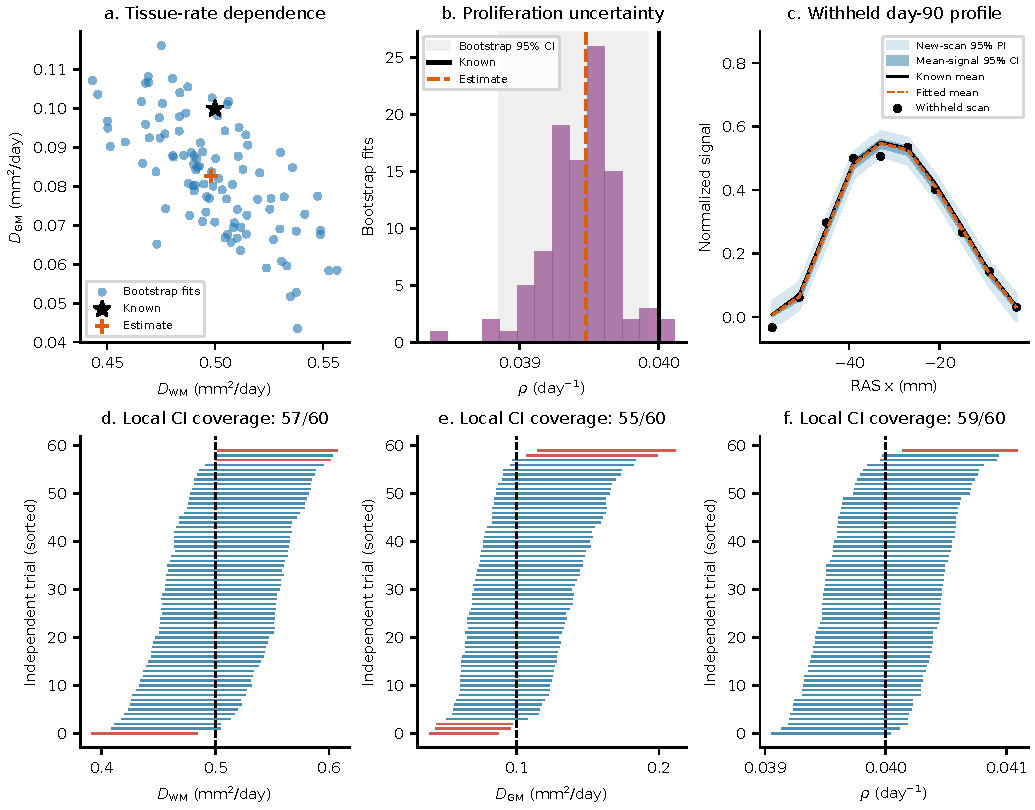
\includegraphics[width=\textwidth]{figures/brainweb_recovery.pdf}
\caption{BrainWeb recovery and conditional uncertainty. (a) Joint white-/gray-matter bootstrap estimates; the star denotes known rates and the cross the primary estimate. (b) Proliferation bootstrap distribution, with marginal percentile interval shading; its known value is just beyond the upper limit. (c) Withheld day-90 profile through the nearest observation-voxel centers to the seed's $y,z$ coordinates. Mean-signal confidence and new-scan prediction intervals are pointwise and have different meanings. (d--f) Local 95\% intervals for 60 independent noise realizations, sorted by fitted rate. Red marks a missed known value. These repetitions share anatomy and biology and do not constitute a virtual patient cohort.}\label{fig:bw_recovery}
\end{figure}

\subsection{BrainWeb withheld forecasts and anatomy sensitivity}\label{sec:bw_sensitivity}
Day-90 RMSE against the noise-free signal was \BWDayNinetyRMSE{} over the full FOV and \BWNearDayNinetyRMSE{} in the prespecified near-seed region (Table~\ref{tab:bw_forecast}). New-scan prediction intervals contained 94.2\% of all withheld day-90 voxels but only 89.2\% of near-seed voxels. Thus, background-inclusive summaries can conceal less favorable performance near the tumor. These are descriptive spatial fractions for one noisy scan, not independent coverage trials or simultaneous spatial guarantees.

\begin{table}[tbp]
\centering\small
\caption{Withheld BrainWeb forecast metrics. The full FOV contains 1,000 observation voxels; the near-seed region contains 120. Errors use normalized signal units. The final column is the spatial fraction of noisy observations in approximate pointwise 95\% new-scan prediction intervals.}\label{tab:bw_forecast}
\begin{tabularx}{\textwidth}{rlYYY}
\toprule Day & Region & RMSE vs clean & RMSE vs noisy & Voxel fraction in prediction interval\\\midrule
\BWForecastRows
\bottomrule
\end{tabularx}
\end{table}

On the shared 3 mm anatomy, changing the maximum step from 0.5 to 0.25 day reduced day-90 signal RMSE relative to the 0.125-day generator from \BWDayNinetyTimeRMSE{} to \BWHalfTimeRMSE{}. By contrast, the 3 mm versus 2 mm generator discrepancy at the known rates reached \BWDayNinetyGridRMSE{} at day 90, or 18.4\% of the 0.02 noise standard deviation (Figure~\ref{fig:bw_anatomy}). This is a change in discretized anatomy and numerical representation rather than a pure spatial-convergence comparison.

Fitting the noise-free 2 mm signal with the 3 mm model estimated $D_{\rm GM}=\BWGrayStressEstimate$ mm$^2$/day, a +\BWGrayStressShift\% shift from the known value (Table~\ref{tab:bw_anatomy}). Corresponding white-matter and proliferation shifts were +0.04\% and -0.13\%. The paired noisy stress fit gave $(0.499160,0.096770,0.039445)$ in the respective units. Its conditional local intervals do not incorporate anatomy/grid discrepancy. Signal error below one noise standard deviation per voxel can therefore coexist with a material rate shift when systematic differences are fitted across many measurements. This sensitivity example does not estimate segmentation uncertainty or establish a universal gray-matter bias.

\begin{table}[tbp]
\centering\small
\caption{Anatomy/grid sensitivity: full 2 mm data fitted with the 3 mm model. The noiseless fit isolates a deterministic rate shift under the changed representation. The noisy fit reuses the primary observation-noise draw. Neither fit estimates a distribution of anatomy uncertainty.}\label{tab:bw_anatomy}
\setlength{\tabcolsep}{3pt}
\begin{tabularx}{\textwidth}{lrrrY}
\toprule Parameter & Known & Noiseless fit & Relative shift & Paired noisy fit\\\midrule
\BWAnatomyRows
\bottomrule
\end{tabularx}
\end{table}

\begin{figure}[p]
\centering
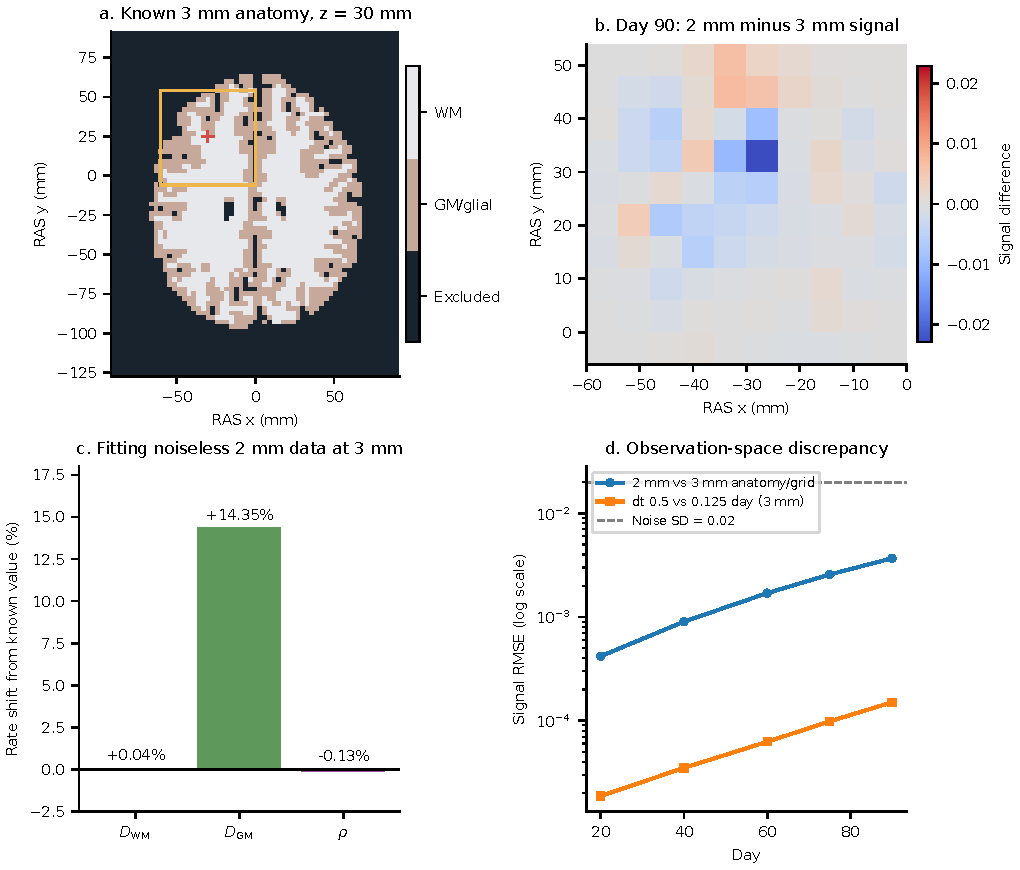
\includegraphics[width=\textwidth]{figures/brainweb_anatomy_sensitivity.pdf}
\caption{Sensitivity to anatomy and numerical representation. (a) Full 3 mm tissue domain at RAS $z=30$ mm, with the known seed center and fixed 60 mm observation FOV. The forward PDE is not cropped to that box. (b) Difference between 2 mm and 3 mm noise-free generating signals at day 90, using identical physical observation voxels; the displayed observation plane is at $z=27$ mm. (c) Relative shifts after fitting the noise-free 2 mm data with the 3 mm inverse model. (d) Observation-space discrepancies at the known rates; temporal error on the shared 3 mm grid is smaller than the combined anatomy/grid effect. Both generators in the anatomy comparison use a 0.125-day step. No biological measurement or clinical validation is represented.}\label{fig:bw_anatomy}
\end{figure}

The two phantom recovery experiments fit synthetic M0 observations only; the subsequent PAT16 recovery uses its tensor-transport counterpart. The oxygen--necrosis parameters and the dense-seed forward comparisons remain assigned inputs; no patient parameters, oxygen/death rates or clinical predictive errors were estimated.
\FloatBarrier

\subsection{PAT16 conditional MRI-informed comparison}\label{sec:pat16_results}
The shared grid contained $51\times62\times50$ voxels, with 44,667 active tissue voxels and 18,202 eligible directional white-matter voxels. A lesion override included 603 voxels classified as CSF by the healthy-tissue segmentation, using assumed gray-matter transport. Resampled tensor-derived FA correlated with the saved T1-space FA at $r=\PATFAR$; this is transformation consistency, not independent registration validation. Of 180 BOLD frames, 157 remained after censoring. The nuisance design had rank 36, leaving 121 algebraic residual degrees of freedom. These counts do not correct for temporal autocorrelation or quantify FC reliability.

Day-90 marginal median normalized burden was 110.42 mL equivalents for isotropic and 106.74 for anisotropic transport (Table~\ref{tab:pat16_outcomes}). The paired median difference was $\PATBurdenDifference$ mL equivalents, with 5th--95th percentiles $[-6.80,-0.85]$. For the illustrative $u\geq0.16$ volume, the paired difference was $-6.36$ mL, with percentiles $[-12.83,-2.46]$. A paired-difference median is computed scenario by scenario and need not equal the difference of the two marginal medians. These are simulated, parameter-dependent effects, not observed changes in the patient.

\begin{table}[tbp]
\centering\small
\caption{PAT16 day-90 conditional outcomes: median [5th, 95th percentile] across \PATScenarios{} paired assumed-parameter scenarios. Differences are anisotropic minus isotropic. The bands are empirical sensitivity ranges, not calibrated patient intervals; the density threshold has no validated MRI correspondence.}\label{tab:pat16_outcomes}
\setlength{\tabcolsep}{3pt}
\begin{tabularx}{\textwidth}{Y Y Y Y}
\toprule Quantity & Isotropic & Anisotropic & Paired difference\\\midrule
\PATRows
\bottomrule
\end{tabularx}
\end{table}

\begin{figure}[p]
\centering
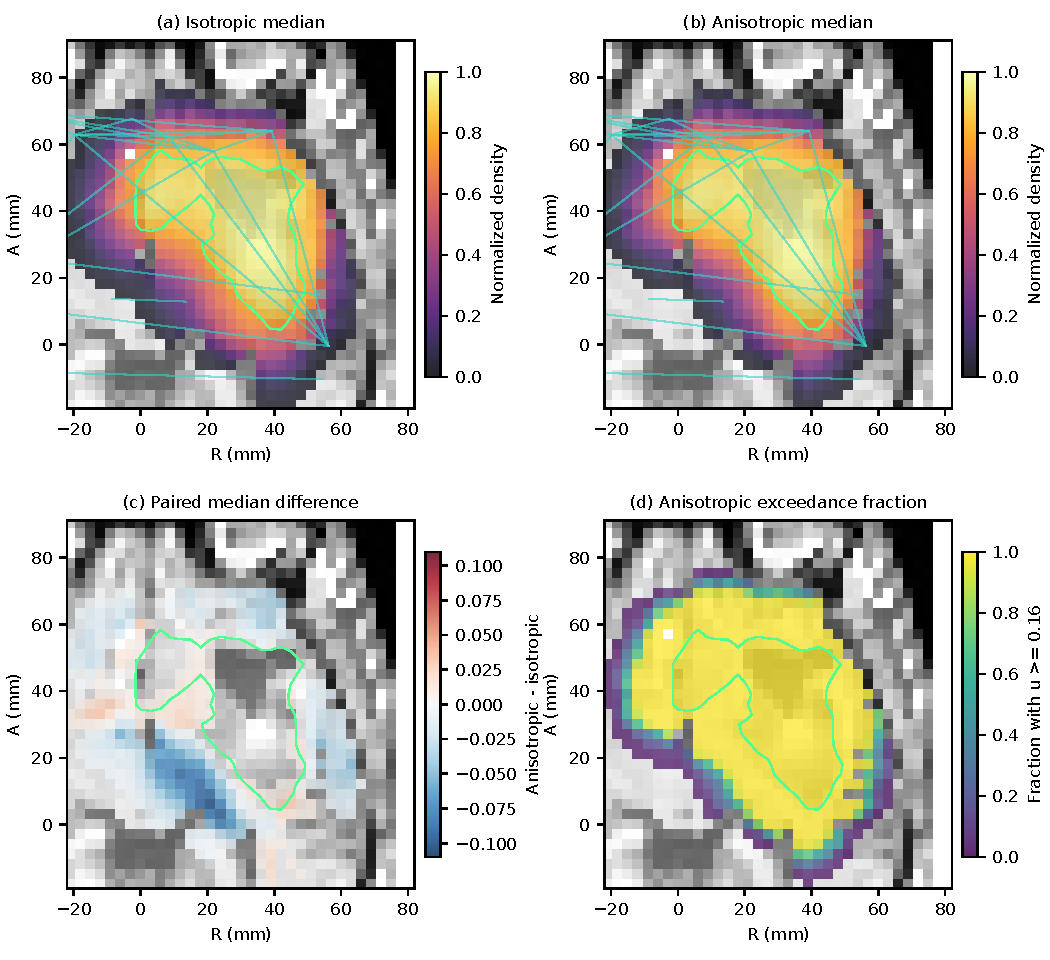
\includegraphics[width=\textwidth]{figures/pat16_fields.pdf}
\caption{PAT16 conditional day-90 growth on the preoperative axial plane at RAS $z=-12$ mm. (a,b) Pointwise marginal median normalized density with shared colors. (c) Median of paired anisotropic-minus-isotropic fields, with the full displayed difference range retained. (d) Fraction of assumed scenarios exceeding $u=0.16$, not a calibrated probability of tumor presence. Green contours show the input lesion at threshold 0.5. Cyan/purple lines in (a,b) are measured positive/negative FC projected from ROI centers within a $\pm12$ mm slab, not anatomical tracts on the slice. Background T1, lesion and FC are measurement-derived; growth is simulated. No functional decline is predicted. Values below 0.02 (absolute difference below 0.005 in panel c) are transparent for display only.}\label{fig:pat16_fields}
\end{figure}

The spatial comparison shows redistribution associated with directional transport (Figure~\ref{fig:pat16_fields}). Marginal global bands substantially overlapped throughout the run (Figure~\ref{fig:pat16_curves}). Regional mean-density summaries and measured static connectivity are supplied with the notebook; they do not constitute network or cognitive forecasts. No later patient scan was used to evaluate the hypothetical untreated evolution.

All paired initial states matched, and recorded densities remained between zero and 0.99733 without clipping. Every scenario used a 0.5-day step. For a representative central anisotropic scenario, halving the step changed day-90 density by \PATTimeDifference\% in relative $L^1$. A five-day pure-diffusion test gave relative mass error $5.69\times10^{-10}$ after float32 output storage. Additional tests verify tensor reconstruction and mixed derivatives, isotropic equivalence, a rotated Gaussian's covariance growth, coordinate transforms, conservation and blocked-corner behavior. These checks support implementation correctness and limited temporal sensitivity; spatial convergence on the PAT16 tissue graph and independent patient prediction have not been demonstrated.

\begin{figure}[tbp]
\centering
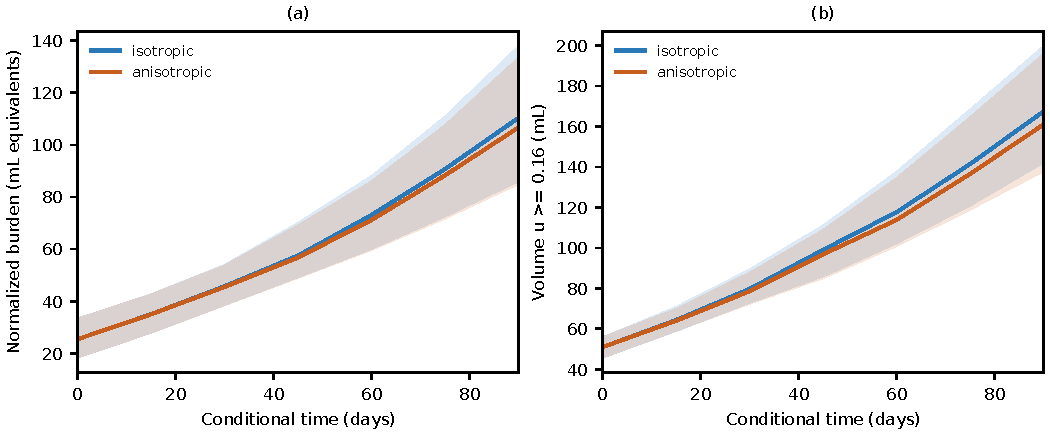
\includegraphics[width=\textwidth]{figures/pat16_timecourses.pdf}
\caption{PAT16 simulated normalized burden and illustrative threshold-defined volume. Lines are marginal medians and shading denotes 5th--95th empirical percentiles over the same \PATScenarios{} paired assumed scenarios. Time zero is lesion-based initialization, not tumor onset. No surgery, radiation, drug effect or oxygen limitation is included. Wide overlapping marginal bands coexist with the negative paired differences in Table~\ref{tab:pat16_outcomes}.}\label{fig:pat16_curves}
\end{figure}
\FloatBarrier

\subsection{PAT16 four-parameter recovery and conditional uncertainty}\label{sec:pat16_recovery_results}
The three starts converged to practically identical estimates. The fitted $(D_{\rm WM},D_{\rm GM},\rho,r)$ was $(\PRWhiteEstimate,\PRGrayEstimate,\PRRhoEstimate,\PRRatioEstimate)$ (Table~\ref{tab:pat16_recovery}). Relative errors were $\PRWhiteError\%$, $\PRGrayError\%$, $\PRRhoError\%$ and $\PRRatioError\%$, respectively. All four generating values lay inside both local and bootstrap marginal 95\% intervals. This does not imply joint 95\% coverage of the four-dimensional parameter vector. No primary, bootstrap or independent-noise fit failed or reached a search bound. These results concern generated signals on patient-derived anatomy; they do not recover biological rates from PAT16 measurements.

\begin{table}[tbp]
\centering\small
\caption{Synthetic four-parameter recovery on PAT16 anatomy. Marginal intervals condition on fixed anatomy, dMRI directions, normalized initialization and signal/noise calibration. They do not estimate absolute capacity. The original pilot's sensitivity percentiles are a separate uncertainty construction.}\label{tab:pat16_recovery}
\setlength{\tabcolsep}{3pt}
\begin{tabularx}{\textwidth}{lrrYY}
\toprule Parameter & Known & Estimate & Local 95\% CI & Bootstrap 95\% CI\\\midrule
\PRRecoveryRows
\bottomrule
\end{tabularx}
\end{table}

WM diffusivity and anisotropy were positively dependent, with local log-parameter correlation \PRWMRatioCorrelation{} (Figure~\ref{fig:pat16_recovery}b,c). Weighted Jacobian singular values were approximately \PRSingularValues{}, with condition number \PRCondition{}. Training standardized residual RMS was \PRTrainingRMS{}. These diagnostics support local estimation under this initialization and observation design, without establishing global identifiability or robustness to unknown directions and initial density.

\begin{figure}[p]
\centering
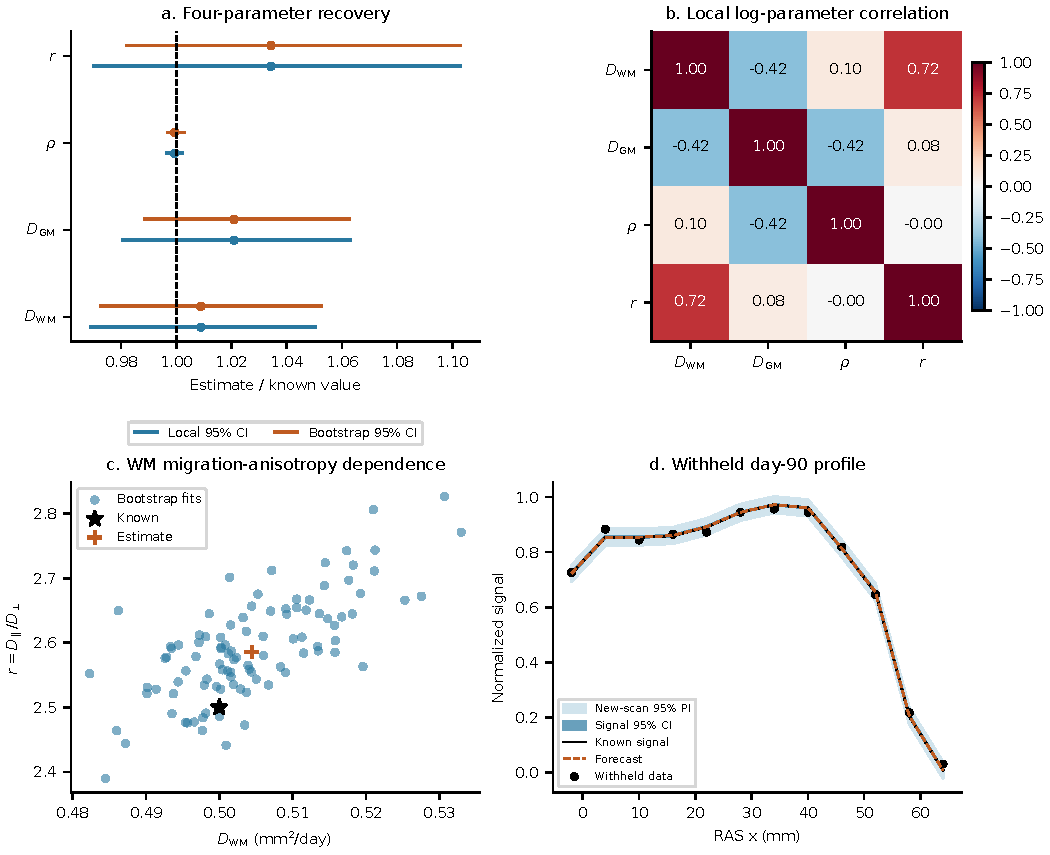
\includegraphics[width=\textwidth]{figures/pat16_recovery.pdf}
\caption{PAT16 synthetic recovery and uncertainty. (a) Primary estimates divided by the known generating values, with local and bootstrap marginal 95\% confidence intervals; the dashed line denotes truth. (b) Local log-parameter correlations. (c) All \PRBootstraps{} bootstrap WM-diffusivity/anisotropy pairs, with known values and the primary estimate. (d) A fixed central observation-voxel row at withheld day 90, showing nominal pointwise 95\% signal confidence and Gaussian-mixture new-measurement prediction intervals. The observation row uses $y=\PRProfileY$, $z=\PRProfileZ$ mm in RAS coordinates. No later measurement enters fitting or resampling. The joint dependence should be propagated; separate marginal endpoints do not define independent parameter combinations.}\label{fig:pat16_recovery}
\end{figure}

Across \PRTrials{} independent noise datasets, marginal local-interval coverage was \PRWhiteCoverage/\PRTrials{}, \PRGrayCoverage/\PRTrials{}, \PRRhoCoverage/\PRTrials{} and \PRRatioCoverage/\PRTrials{} (Table~\ref{tab:pat16_recovery_coverage}; Figure~\ref{fig:pat16_recovery_validation}). Mean relative biases were $\PRWhiteBias\%$, $\PRGrayBias\%$, $\PRRhoBias\%$ and $\PRRatioBias\%$. Exact binomial intervals contained the nominal 95\% level but remained broad; this is not evidence of established 95\% calibration. The audit includes the declared temporal mismatch while holding anatomy, directions, initialization and observation calibration fixed. It does not assess marginal bootstrap parameter-interval coverage or robustness to broader model error.

\begin{table}[tbp]
\centering\small
\caption{PAT16 independent-noise audit of local 95\% intervals. Bias is relative to the known parameter; RMSE uses the parameter's units. Exact binomial intervals quantify Monte Carlo uncertainty in coverage. Failed/boundary intervals would count as misses; none occurred.}\label{tab:pat16_recovery_coverage}
\setlength{\tabcolsep}{3pt}
\begin{tabularx}{\textwidth}{lrrYY}
\toprule Parameter & Mean bias & RMSE & Local coverage & Exact 95\% binomial CI\\\midrule
\PRCoverageRows
\bottomrule
\end{tabularx}
\end{table}

\begin{figure}[p]
\centering
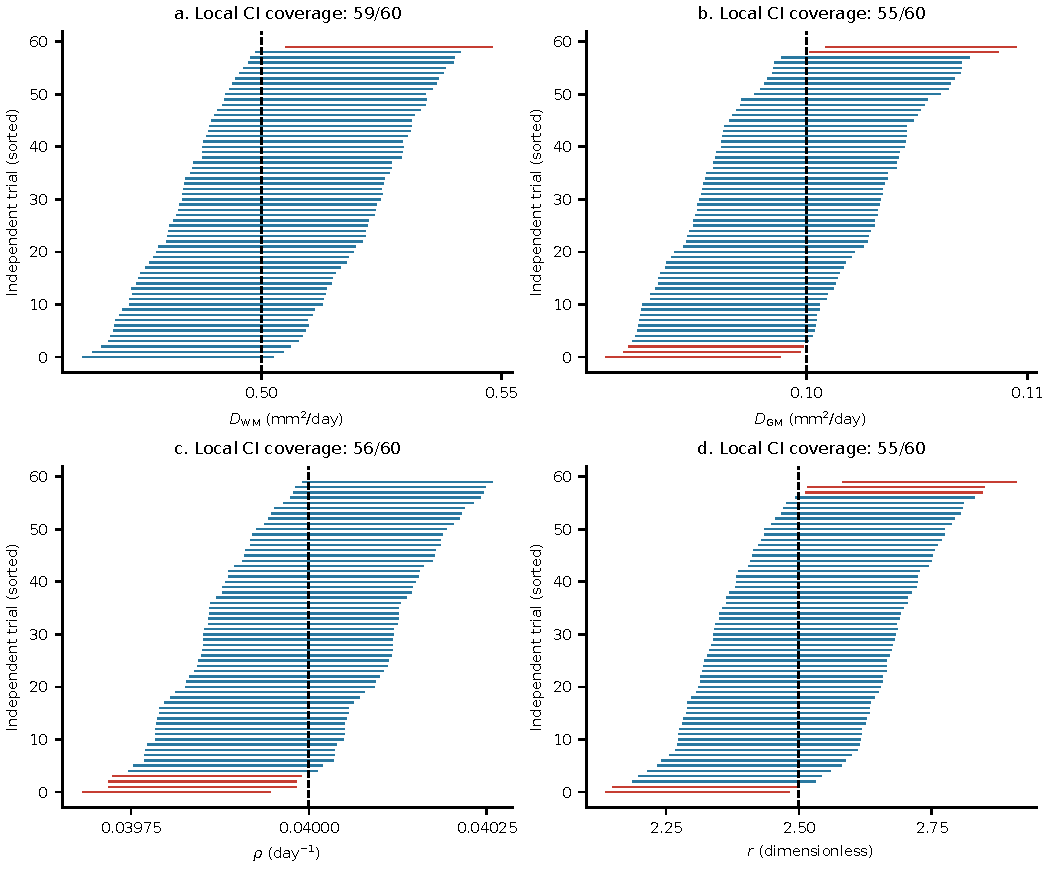
\includegraphics[width=\textwidth]{figures/pat16_recovery_validation.pdf}
\caption{Validation against known synthetic generating parameters on PAT16 anatomy across \PRTrials{} fresh noise datasets. Each segment is a marginal local 95\% interval, sorted within parameter by fitted value; the black dashed line is the known value. Red intervals miss truth. Counts include all attempted trials. These repetitions share anatomy, initialization, directions, biology and observation calibration; they are independent noise realizations, not independent patients. Exact binomial intervals and parameter bias/RMSE are reported in Table~\ref{tab:pat16_recovery_coverage}.}\label{fig:pat16_recovery_validation}
\end{figure}

\subsection{PAT16 withheld forecasts and numerical validation}\label{sec:pat16_recovery_forecast}
Full-cube forecast RMSE against the noise-free signal was \PRDaySeventyFiveRMSE{} at day 75 and \PRDayNinetyRMSE{} at day 90, while noisy-scan RMSE was approximately the assumed 0.015 noise standard deviation (Table~\ref{tab:pat16_recovery_forecast}). The nominal pointwise 95\% signal intervals contained \PRDaySeventyFiveSignalContainment\% and \PRDayNinetySignalContainment\% of full-cube truth values. Final Gaussian-mixture prediction intervals contained \PRDaySeventyFivePredictionContainment\% and \PRDayNinetyPredictionContainment\% of noisy observations; near-center fractions were \PRNearDaySeventyFivePredictionContainment\% and \PRNearDayNinetyPredictionContainment\%. These descriptive spatial fractions do not establish repeated or simultaneous coverage.

Mean full-cube signal-interval widths were \PRDaySeventyFiveSignalWidth{} and \PRDayNinetySignalWidth{}; final prediction widths were \PRDaySeventyFivePredictionWidth{} and \PRDayNinetyPredictionWidth{} normalized signal units at days 75/90. The original 100 noisy draws gave about 93.2\%/93.1\% containment and widths 0.05642/0.05639. Increasing predictive draws to 1,000 and \PPDraws{} reduced interval-endpoint RMSE against the integrated mixture from \PPEndpointLegacy{} to \PPEndpointThousand{} and \PPEndpointMany{}, respectively (Figure~\ref{fig:pat16_prediction_validation}a). Integration removes noise-tail sampling error without tuning widths; the number of distinct parameter vectors remains \PRBootstraps{}.

\begin{table}[tbp]
\centering\small
\caption{Withheld PAT16 forecast validation. The full FOV contains 1,728 observation voxels and the near-center sphere 280. Signal RMSE is against noise-free truth. The noisy RMSE is divided by the known noise SD. The last two columns report spatial containment in nominal pointwise 95\% signal confidence and Gaussian-mixture new-observation prediction intervals, respectively. These fractions are not an independent coverage audit.}\label{tab:pat16_recovery_forecast}
\setlength{\tabcolsep}{3pt}
\begin{tabularx}{\textwidth}{rlYYYY}
\toprule Day & Region & Signal RMSE & Noisy RMSE/SD & Truth in signal CI & Data in prediction interval\\\midrule
\PRForecastRows
\bottomrule
\end{tabularx}
\end{table}

Across \PPTrials{} independently regenerated datasets and \PPNestedFits{} nested bootstrap refits, full-cube mean coverage was \PPOldFullSeventyFive\%/\PPOldFullNinety\% for 100 noisy draws, \PPManyFullSeventyFive\%/\PPManyFullNinety\% for \PPDraws{} draws and \PPMixFullSeventyFive\%/\PPMixFullNinety\% for integrated intervals at days 75/90 (Table~\ref{tab:pat16_prediction_validation}). The integrated mean-coverage Monte Carlo 95\% intervals were \PPMixFullSeventyFiveCI\% and \PPMixFullNinetyCI\%; near-center mean coverage was \PPMixNearSeventyFive\% and \PPMixNearNinety\%. Day-75 full-cube coverage was slightly conservative: its Monte Carlo lower limit lay just above 95\%, rather than demonstrating exact nominal calibration. Paired full-cube coverage gains over 100 noisy draws were \PPGainSeventyFive{} percentage points (MC 95\% interval \PPGainSeventyFiveCI{}) and \PPGainNinety{} (\PPGainNinetyCI{}) at days 75/90. Widths and interval scores distinguish improvement in tail estimation from point accuracy, which is shared by the methods.

Every primary and nested fit succeeded without a boundary optimum. At the prespecified central voxel, integrated intervals covered \PPSentinelSeventyFive/\PPTrials{} and \PPSentinelNinety/\PPTrials{} fresh observations, with exact binomial 95\% limits \PPSentinelSeventyFiveCI\% and \PPSentinelNinetyCI\%. These broad limits leave single-voxel calibration uncertain. Regional averages support near-nominal pointwise coverage for this fixed design; coverage at each location, under model error or in patients remains unestablished.

\begin{table}[p]
\centering\small
\caption{Repeated PAT16 prediction-interval validation. Each of \PPTrials{} independent datasets refits the four rates and 100 bootstrap samples. Coverage is the mean within-image fraction; bracketed 95\% Monte Carlo limits use dataset-level Student-$t$ uncertainty, avoiding pooled-voxel independence. Width and the proper interval score are in normalized signal units; lower score is better. The score adds $2/0.05$ times the distance of an observation outside the interval to its width. All attempted datasets are included.}\label{tab:pat16_prediction_validation}
\setlength{\tabcolsep}{3pt}
\begin{tabularx}{\textwidth}{lrlYrr}
\toprule Method & Day & Region & Coverage [MC 95\% CI] (\%) & Width & Score\\\midrule
\PPValidationRows
\bottomrule
\end{tabularx}
\end{table}

\begin{figure}[p]
\centering
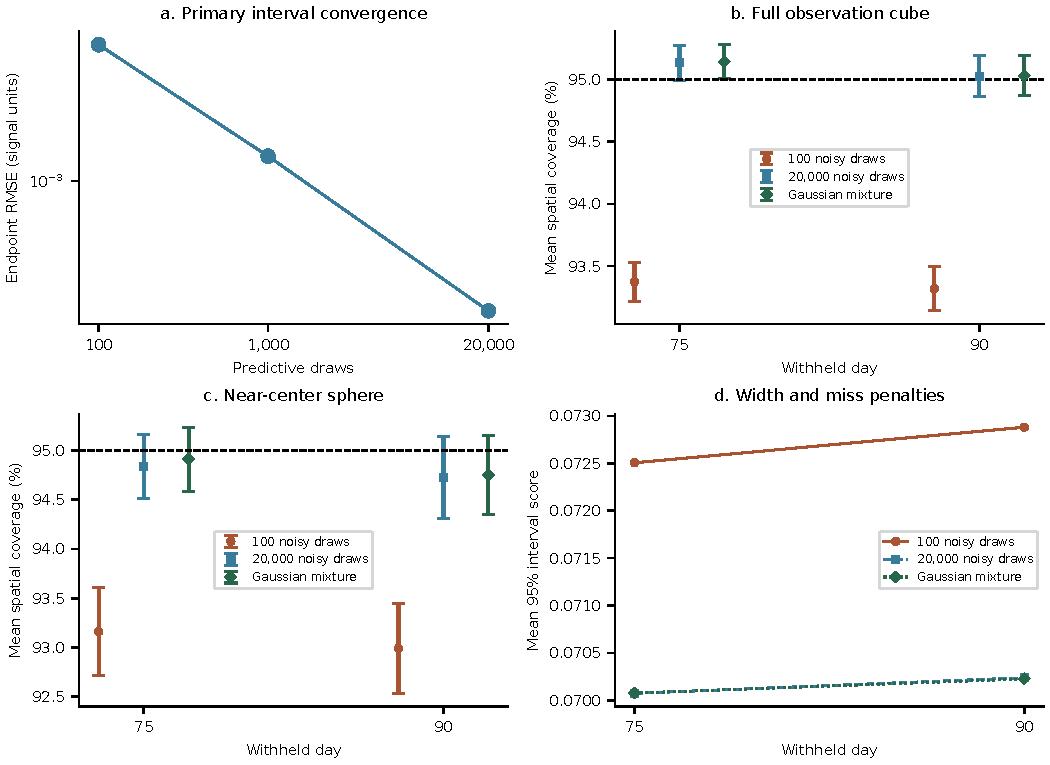
\includegraphics[width=\textwidth]{figures/pat16_prediction_validation.pdf}
\caption{Improved PAT16 pointwise 95\% prediction intervals. (a) Primary endpoint RMSE relative to Gaussian-mixture quantiles, over both tails, withheld days and all observation voxels; 100 draws use the legacy construction, while 1,000/20,000 draws resample bootstrap trajectories. (b,c) Mean spatial coverage across \PPTrials{} fresh datasets, with dataset-level Monte Carlo 95\% limits; the dashed line is nominal coverage. (d) Mean full-cube proper interval score, penalizing width and misses. Each repetition independently refits the early data and 100 bootstrap datasets; future noise is independent of training and resampling. Gaussian integration removes predictive noise sampling error, while uncertainty from finite bootstrap fits and the fixed model remains.}\label{fig:pat16_prediction_validation}
\end{figure}

The noise-free matched-model fit recovered all four generating values with maximum relative error \PRMatchedError{}; this is a matched-discretization implementation check. Fitting noise-free finer-time signals shifted WM diffusion, GM diffusion, proliferation and anisotropy by $\PRWhiteTemporalShift\%$, $\PRGrayTemporalShift\%$, $\PRRhoTemporalShift\%$ and $\PRRatioTemporalShift\%$, respectively. Thus the largest temporal-mismatch shift was \PRTemporalMaxShift\%. These deterministic shifts are outside the sampling-interval construction. The check retained the spatial anatomy and stencil and cannot establish spatial convergence. Time-zero-only inference was correctly rejected. Tests also rejected four-parameter fitting without directional information or with only one tissue class. Conditional numerical recovery and synthetic forecasting do not validate the patient observation model or biological migration anisotropy.

\begin{figure}[p]
\centering
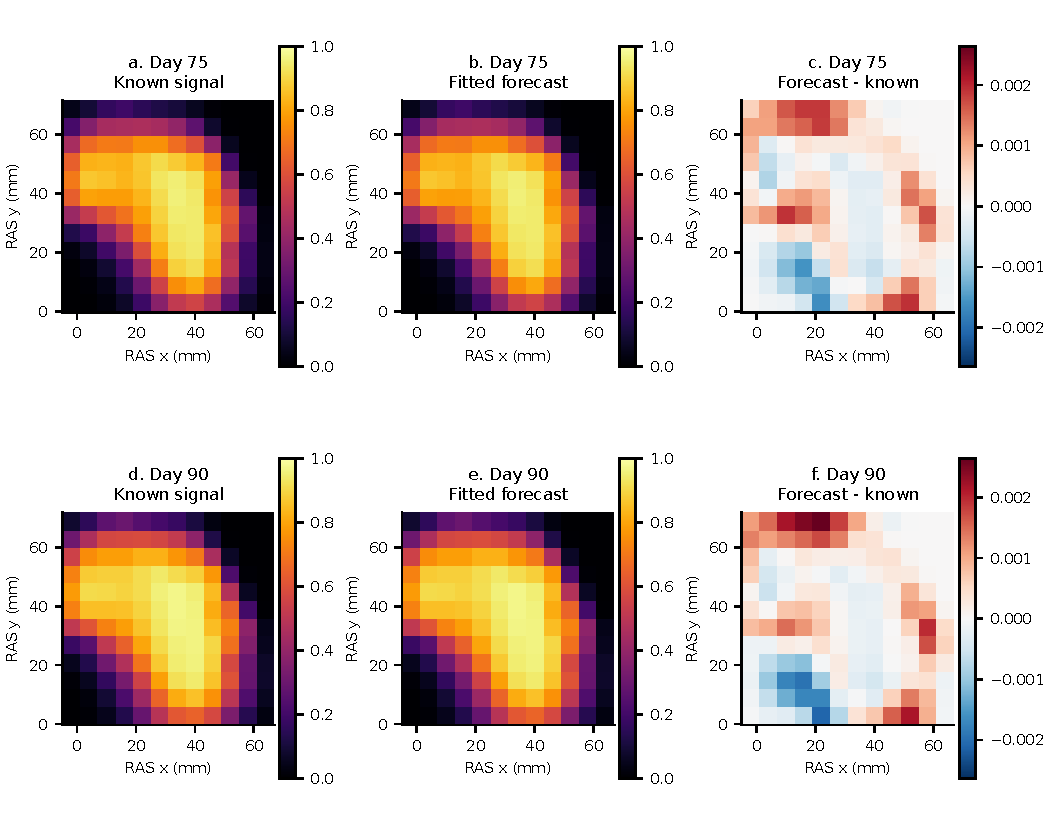
\includegraphics[width=\textwidth]{figures/pat16_recovery_forecast.pdf}
\caption{PAT16 withheld day-75 (top) and day-90 (bottom) noise-free signals on the central observation plane, RAS $z=\PRProfileZ$ mm. Left: known synthetic signal. Middle: the forecast calibrated only at days 20/40/60. Right: fitted minus known signal, with one shared symmetric residual range retaining all displayed errors. The known and fitted signals share a $0$--$1$ scale. Each pixel approximates a 6 mm cube average after Gaussian blur with 2 mm standard deviation; these are synthetic signals, not patient MRI intensities or a fine-grid tumor-density slice. Pointwise interval behavior is shown in Figure~\ref{fig:pat16_recovery}d and Table~\ref{tab:pat16_recovery_forecast}.}\label{fig:pat16_recovery_forecast}
\end{figure}
\FloatBarrier

